\documentclass[../journal_main.tex]{subfiles}
\begin{document}

\chapter{Monte Carlo simulations}
The purpose of this chapter is to give a brief introduction to Monte Carlo simulations and their applications in the numerical analysis of phase transitions in statistical physics models. We will start by illustrating the general idea of importance sampling Monte Carlo methods, followed by the different type of update schemes (Metropolis, Wolff-cluster, etc.) to sample non-uniform distributions efficiently. We will also pay attention to the topic of statistical analysis of the generated data via autocorrelation analysis and statistical error analysis. For illustration purposes, we will primarily focus our attention on the simplest spin model, i.e., the two-dimensional Ising model (without external field) and discuss the finite-temperature critical phenomena and phase transition. Finally, we will demonstrate the calculation of the critical exponents of the two-dimensional Ising model using finite-size scaling analysis of relevant physical observables. Although we start with a classical statistical model, these ideas can be generalized and are applicable in simulations of quantum-spin systems, where they become the \textit{Quantum Monte Carlo} (QMC) methods [Janke, Sandvik]. 

\section{Introduction to Monte Carlo}
Monte Carlo simulations are an important and broad class of stochastic methods that utilize randomness to solve deterministic problems efficiently. To show their utility, we will start with a simple and illustrative example. Consider the calculation of a thermal expectation value of an observable $Q(x)$ in statistical physics;
\begin{equation}
    \expval{Q} = \int_0^L \dd x \: \rho(x) Q(x), \qquad \qquad \int_0^L \dd x \: \rho(x) = 1,
    \label{sample_integral}
\end{equation} 
where $\rho(x)$ is the underlying probability distribution.~\\~\\
The most naive way to estimate this integral numerically is to use \textit{Euler's method}  to discretize the integration range into $N$ pieces and perform a discretized sum
\begin{equation}
    \expval{Q} \approx \Delta x \sum_{j=1}^N \rho(x_0 + j \Delta x) \: Q(x_0 + j\Delta x)
\end{equation} 
where $\Delta x = L/N$. Such grid-based methods are very accurate for low-dimensional integrals, but as we go to higher-dimensional integrals, both the error-scaling and computational costs grow significantly.~\\~\\
A more efficient method for performing high-dimensional integrals is known as \textit{Monte Carlo integration} where the points are uniformly sampled across the integration range instead of a grid. If the uniformly sampled random points are denoted by the set $\{x_1, x_2, x_3, \ldots, x_N \}$, then the integral in Eq. \eqref{sample_integral} can be estimated as 
\begin{equation}
    \expval{Q} \approx \frac{L}{N} \sum_{i=1}^N \rho(x_i) \: Q(x_i)
\end{equation} 
The error in a Monte Carlo estimate goes as $1/\sqrt{N}$ in any number of dimensions, and hence it is more efficient for estimating $6 \mathcal{N}$-dimensional integrals characteristic of statistical mechanics of $\mathcal{N}$ particles. However, this straightforward unbiased Monte Carlo integration only works well in practice if the integrand isn't sharply peaked in some small region of the integration range.
%%% FIG %%%
\begin{figure}[!htb]
    \centering
    \begin{subfigure}[b]{1.0\textwidth}  %keep total sum <1 to show in same line
        \centering
        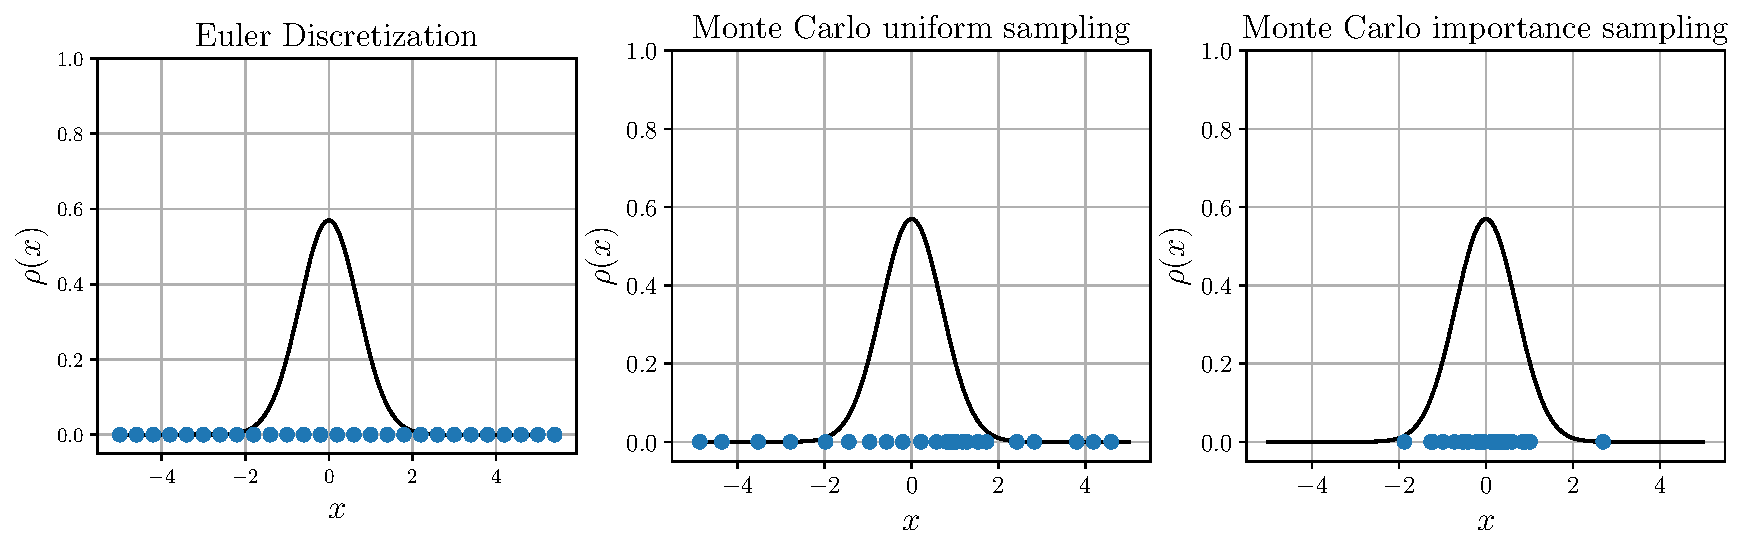
\includegraphics[width=\textwidth]{images/monte_carlo/sampling.pdf}
    \end{subfigure}
    \caption{Comparision of sampling techniques.}
    \label{}
\end{figure}
%%% FIG %%%
\FloatBarrier \!\!\!\!\!\!\!\!\!\!\!
If $\rho(x)$ is sharply peaked in a small region, then uniform sampling of points can result in large statistical fluctuations as only a small fraction of points will fall within the dominant range. Therefore, the next improvement can be performed by sampling the points according to a probability distribution $W(x)$ which is peaked in the same region as $\rho(x)$. This gives the estimate of the expectation value as 
\begin{equation}
    \expval{Q} \approx \frac{L}{N} \sum_{i=1}^N \frac{\rho(x_i)}{W(x_i)} Q(x_i) \: W(x_i) \approx \frac{1}{N} \sum_{i=1}^N {}^{{}^{(W)}} \frac{\rho(x_i)}{W(x_i)} \: Q(x_i)
\end{equation}  
where $\sum {}^{(W)}$ denotes points being sampled from the distribution $W(x)$, and we write $L \sum W(x_i) \to \sum {{}^{(W)}}$. Often, a good solution is to use $W(x) = \rho(x)$, and the expectation value becomes an arithmetic average of $Q(x)$ over the configurations sampled by $\rho(x)$
\begin{equation}
    \expval{Q} \approx \frac{1}{N} \sum_{i=1}^N {}^{{}^{(\rho)}} Q(x_i)
\end{equation}
This technique is known as the \textit{Monte Carlo Importance Sampling} method since we are only sampling the points lying in the ``important'' region of the probability distribution $\rho(x)$.~\\~\\
In statistical mechanics, the probability distribution is generally the Boltzmann distribution $\rho(\vec{x}, \vec{p}) = e^{-\beta H (\vec{x},\vec{p})}$, and we can use Monte Carlo importance sampling to calculate expectation values of physical observables. However, in the above discussion, we have ignored the problem of sampling points according to a given probability distribution. We discuss this in the following subsection.

\subsection{Detailed Balance condition}
In order to calculate integrals via the method of importance sampling, we need a way to sample points according to the probability distribution $\rho(x)$. The theory of Markov Chains provides us with the necessary tools to generate a Markov Chain process which evolves towards a desired equilibrium distribution.~\\~\\
In physicists' language, a Markov chain is a discrete chain of events $C_1 \to C_2 \to C_3 \to \ldots \to C_N$ that evolves stochastically and satisfies the Markovian property, i.e., the probability of $C_{i-1} \to C_i$ transition is independent of its history. Put together, this implies the probability of obtaining the above sequence is
\begin{equation}
    P(C_1 \to C_2 \to\ldots \to C_N) = P(C_1)\cdot P(C_2 | C_1) \cdot P(C_3 | C_2) \ldots P(C_N | C_{N-1})
\end{equation}
Roughly speaking, if the Markov chain doesn't repeat itself and can reach \textit{any}  configuration starting from \textit{any other}  configuration, then it is \textit{ergodic} and settles onto a stationary distribution. By designing an appropriate Markov chain, it is possible to obtain any desired stationary distribution $\rho(C)$ .~\\~\\
Let us now assume we have a set of all possible configurations $\{X\} = \{X_1, X_2, \ldots, X_n\}$ in the configuration space. Assume we start with some configuration $X_{i(0)}$ and stochastically generate a Markov chain $X_{i(1)}, X_{i(2)}, X_{i(3)}, \ldots, X_{i(M)}$. We can do the same for an ensemble of configurations initially distributed according to $\rho(X)$. At the update $0$ , the number of configurations $X_i$ in the initial ensemble is $N_0(X_i) \: \propto \: \rho(X_i) \Rightarrow N_0 (X_i) = \mathcal{N} \rho(X_i)$. The given Markov chain must have an update scheme which stochastically evolves the ensemble to the next set of states. The number of configurations after the update $1$ is
\begin{equation}
    N_1(X_i) = N_0(X_i) + \sum_{j\neq i} \qty[N_0(X_j) \: P(X_j \to X_i) - N_0(C_i) \: P(X_i \to X_j)]
    \label{master}
\end{equation}
The first term in the sum represents configurations updating into $X_i$ and the second term represents $X_i$ updating out to other configurations. If we want the ensemble to remain distributed according to the initial ensemble distribution $\rho(X)$, then, for all $i = 1, 2, \ldots M$,
\begin{equation}
    \sum_{j\neq i} \qty[\rho(X_j) \: P(X_j \to X_i) - \rho(C_i) \: P(X_i \to X_j)] \stackrel{!}{=} 0
\end{equation}  
One possible solution of this condition is to satisfy it term-by-term $\forall \: \: j$ 
\begin{equation}
    \rho(X_j) \: P(X_j \to X_i) - \rho(C_i) \: P(X_i \to X_j) \stackrel{!}{=} 0
\end{equation}
which can be written as a ratio 
\begin{equation}
    \frac{P(X_j \to X_i)}{P(X_i \to X_j)} = \frac{\rho(X_i)}{\rho(X_j)},
    \label{detailedbalance}
\end{equation}
also known as the \textit{detailed balance condition}. Although here we start with an ensemble distributed according to the probability distribution $\rho$, for practical purposes, neither do we need to start from the same distribution, nor do we require an ensemble of configurations. In practice, the master equation Eq. \eqref{master} takes care of the excess or deficiency and equilibrates after a characteristic \textit{equilibration time} of Markov chain updates.~\\~\\
The transition probability $P(X_i \to X_j)$ can further be written as a product of the update proposal and the proposal acceptance probabilities 
\begin{equation}
    P(X_i \to X_j) = \underbrace{\mathcal{A}(X_i \to X_j)}_{\text{propose }X_i \to X_j} \cdot \underbrace{P_\text{accept}(X_i \to X_j)}_{\text{accept }X_i \to X_j}
\end{equation}
Since the proposal probabilities should be uniform $\mathcal{A}(X_i \to X_j) = \text{constant}$ , the detailed balance condition in terms of acceptance probabilities becomes 
\begin{equation}
    \frac{P_\text{accept}(X_j \to X_i)}{P_\text{accept} (X_i \to X_j)} = \frac{\rho(X_i)}{\rho(X_j)}
    \label{detailedbalance_metropolis}
\end{equation}
Starting from the detailed balance condition, one can define stochastic algorithms, such as Monte Carlo simulations, which generate configurations according to a desired distribution. One such common algorithm is the \textit{Metropolis algorithm} with the solution to Eq. \eqref{detailedbalance_metropolis} as 
\begin{equation}
    P_\text{accept}(X_i \to X_j) = \min \qty[\frac{\rho(X_j)}{\rho(X_i)}, 1]
\end{equation}
For statistical mechanics, the desired equilibrium distribution is the Boltzmann distribution which gives rise to the well-known Metropolis acceptance probability
\begin{equation}
    P_\text{accept}(E_i \to E_j) = \min \qty[e^{-\beta(E_j - E_i)}, 1]. 
    \label{metropolis}
\end{equation}

\section{Metropolis and the Ising model}
As discussed in the last section, we can generate samples distributed according to the Boltzmann distribution if we choose the acceptance probability as defined in Eq. \eqref{metropolis} for the Markov chain. These drawn configurations can then be utilized to calculate thermal expectation values via importance sampling.~\\~\\
We will discuss this simulation method in the context of the 2-dimensional ferromagnetic Ising model. The Ising model is the paradigmatic model for systems exhibiting continuous phase transition from a ferromagnetic to a paramagnetic phase at a critical temperature $T_c$. In the absence of an external field $(h=0)$ and only nearest-neighbor interactions, the energy of the ferromagnetic Ising model is 
\begin{equation}
    E = -J \sum_{\expval{i, j}} \sigma_i \sigma_j
    \label{ising}
\end{equation}
where $\expval{i, j}$ indicates nearest-neighbors $i, j$ and the expression for a 2-dimensional square lattice can be more suggestively written as 
\begin{equation}
    E  = -J \sum_{i} \sigma_{i_x, i_y}  \: [\sigma_{i_x, i_y + 1} + \sigma_{i_x + 1, i_y}]
\end{equation}   
For a Markov chain transition $\sigma_i \to - \sigma_i$, the difference in energy between the configurations is given by 
\begin{equation}
    \Delta E = 2J \: \sigma_{i_x, i_y} \: [\sigma_{i_x, i_y + 1} + \sigma_{i_x + 1, i_y} + \sigma_{i_x, i_y - 1} + \sigma_{i_x - 1 , i_y}]
    \label{dE}
\end{equation}
This leads to the Metropolis acceptance probability for the Ising model spin flips being given by
\begin{equation}
    P_\text{accept}(\sigma_i \to -\sigma_i) = \min \qty[e^{-\beta \Delta E}, 1]
    \label{metropolis_ising}
\end{equation}
with $\Delta E$ being defined by Eq. \eqref{dE}. In a nutshell, a \textit{Metropolis Monte Carlo} simulation of the Ising model consists of performing such spin flip proposals by selecting the spin $\sigma_i$ to be flipped at random and generating a Markov chain distributed according to the Boltzmann distribution. A single \textit{Monte Carlo sweep} then consists of $L^2$ such spin flip proposals so that roughly each lattice site gets an equal chance to flip, where $L$ denotes the side length of the square lattice. As a step-by-step procedure, a Monte Carlo sweep is defined as follows:
\begin{enumerate}
    \setlength\itemsep{0.3em}
    \item Randomly choose a spin $\sigma_i$ on the lattice.
    \item Propose the spin flip $\sigma_i \to - \sigma_i$.
    \item Calculate the difference in energy $\Delta E = E_\text{final} - E_\text{initial}$.
    \item Accept the proposed move with a probability of $\min \qty[e^{-\beta \Delta E}, 1]$.
    \item Steps $1$ to $4$ are then repeated $\mathcal{N} = L^2$ times.       
\end{enumerate}
The Boltzmann sampling performed using Markov Chain Monte Carlo (MCMC) can then be utilized in calculating expectation values of observables as simple statistical averages over the sampled points
\begin{equation}
    \expval{\mathcal{O}} \approx \frac{1}{N} \sum_{\{\sigma\}} \mathcal{O(\sigma)}
\end{equation}
where we have suppressed the superscript ${}^{(\rho)}$ on the sum denoting sampling over the distribution $\rho(\{\sigma\}) = e^{-\beta E(\{\sigma\})}$. Note that such Monte Carlo averages are always supposed to be taken over \textit{equilibrated} configurations in a Monte Carlo simulation. As discussed earlier, the master equation \eqref{master} ensures the equilibration of the Markov chain's probability distribution after a few steps by taking care of appropriate excess or deficiencies during the initial steps. This initial equilibration period where no measurements are performed is known as the \textit{equilibration time} or the \textit{thermalization time}, often denoted by $t_\text{eq}$.~\\~\\
The Metropolis MCMC method is thus a conceptually simple and quite universally applicable algorithm. Its applications range from simulations of simple Ising chains to highly non-trivial spin systems. However, the Metropolis algorithm comes with its fair share of problems which we will discuss later. In the next section, we will discuss the relevant statistical physics of the Ising model and the measurement of physical observables.

\section{Physical quantities}
To set the scenery for calculating observable expectation values, we will first begin by discussing the relevant physical observables for the Ising model. Since we are dealing with spin systems, a natural quantity of interest is the magnetization, which acts as the \textit{order parameter} of the Ising phase transition at $T_c \neq 0$. The magnetization per site is defined by the observable
\begin{equation}
    m \equiv \frac{1}{\mathcal{N}} \sum_{i=1}^{\mathcal{N}} \sigma_i
\end{equation} 
where $\mathcal{N}=L^2$ is the total number of lattice sites. One can explicitly check that an operation which rotates all spins $\sigma_i \to -\sigma_i \:\: \forall \: i$ is a symmetry of the Ising Hamiltonian (Eq. \eqref{ising}). Although we are technically not yet dealing with quantum mechanics, this operation can be denoted as $F = \prod_{i=1}^N X_i$ where $X_i$ denotes a flip of spin at site $i$. Since applying this operation twice is equivalent to identity ($F^2 = \mathds{1}$), we often say that the Ising model possesses a global $\mathbb{Z}_2$ symmetry.~\\~\\
As a result of this global $\mathbb{Z}_2$ symmetry, both negative and positive magnetization are equally probable. However, in the thermodynamic limit $\mathcal{N} \to \infty$ (infinitely large lattice), if the system attains a state with spins predominantly in one direction below $T < T_c$, then it cannot spontaneously (in a finite time) fluctuate through a series of local spin flips into a state with the opposite magnetization. This is known as the \textit{spontaneous symmetry-breaking} of the global $\mathbb{Z}_2$ symmetry in the Ising model, and can be physically thought of as arising from the limit of a very weak external field. However, in a finite system, such fluctuations are possible and it is possible for $\expval{m} = 0$ for all temperatures $T$, making it difficult to study the phase transition which appears in the thermodynamic limit.~\\~\\
Therefore, in simulations of finite lattice sizes, \textbf{we instead define the order parameter as} ${\expval{|\boldsymbol{m}|}}$\textbf{.} As the system size increases, the $\expval{|m|}$ curve sharpens close to $T_c$ and approaches the thermodynamic limit symmetry-broken $\expval{m(T)}$ curve.~\\~\\
Similarly, the other relevant physical observable is the energy density which is simply defined as the energy per site
\begin{equation}
    e = \frac{E}{\mathcal{N}} = \frac{-J}{\mathcal{N}} \sum_{\expval{i,j}} \sigma_i \sigma_j
\end{equation}  
We can also use magnetization and energy density observables to calculate other derived quantities of interest. In the context of magnetization, we can calculate the magnetic susceptibility 
\begin{equation}
    \chi \equiv \pdv{\expval{M}}{h}\eval_{h=0}
\end{equation}
i.e. the linear response of magnetization in the weak field limit, i.e.,  $\displaystyle E' = \lim_{h \to 0} (E - hM)$. It is easy to show that the expression for susceptibility simplifies to
\begin{equation}
    \chi = \frac{1}{T}\qty(\expval{M^2} - \expval{|M|}^2) = \frac{L^2}{T}\qty(\expval{m^2} - \expval{|m|}^2)
\end{equation}
where we have replaced the $\expval{m}$ with $\expval{|m|}$ for reasons discussed previously. Similarly, the specific heat capacity is another quantity of interest which is defined as 
\begin{equation}
    C_V = \pdv{\expval{E}}{T} = \frac{L^2}{T^2} \qty(\expval{e^2} - \expval{e}^2)
\end{equation}
Finally, we are also interested in the derived \textit{Binder cumulant} which is defined as the kurtosis of the order parameter $\expval{|m|}$
\begin{equation}
    U_L = 1 - \frac{\expval{m^2}_L}{3\expval{m^2}_L},
\end{equation} 
and the intersection of $U_L$ curves for different lattice side $L$ is used to accurately determine the phase transition point.~\\~\\
Therefore, the measurements of the set of physical observables $\{|m|, m^2, m^4, e, e^2\}$ is sufficient to determine the $Q$ vs. $T$ curves for all the relevant observables $(e, |m|)$  and derived quantities $(\chi, C_V, U_L)$. Using Monte Carlo simulations, we can calculate the expectation values and statistical errors in these quantities, and use the simulation data to extract the critical exponents, which we will discuss in later sections.

\section{Autocorrelation functions}
All MCMC algorithms are based upon the central idea of performing local or cluster updates to arrive at the next configuration (or the next state in a Markov chain). Naturally, it is reasonable to expect that the observable measurements are temporally correlated and these correlations are quite significant near the transition points. The only way to get around this is to perform the measurements of the observables after a few time steps so as to ensure that subsequent measurements are statistically uncorrelated.  The \textit{autocorrelation function} is a quantitative measure of temporal correlations between measurements. For an observable $\mathcal{O}$, the autocorrelation function is defined as
\begin{equation}
    A_\mathcal{O}(t) =   \frac{1}{N-t} \sum_{k=0}^{N-t-1}\frac{\qty(\mathcal{O}(k) - \expval{\mathcal{O}})\cdot\qty(\mathcal{O}(k+t) - \expval{\mathcal{O}})}{\expval{\mathcal{O}^2} - \expval{\mathcal{O}}^2}
    \label{autocorrelationfn}
\end{equation}  
where $\mathcal{O}(k)$'s are the measurements performed at each MC sweep, and $N$ is the total number of MC sampling sweeps. Moreover, the averages in Eq. \eqref{autocorrelationfn} are calculated only over the first $N-t$ measurements. 
\begin{equation}
    \expval{\mathcal{O}^n} = \frac{1}{N-t} \sum_{k=0}^{N-t-1} \qty[\mathcal{O}(k)]^n
\end{equation}
The autocorrelation function is suitably normalized to give values $\in [-1,1]$. For an ergodic simulation, we expect $A_\mathcal{O}(t) \to 0$ as $t \to \infty$; infact, $A_\mathcal{O}(t)$ is expected to fall off as an exponential
\begin{equation}
    A_\mathcal{O}(t) \sim e^{-|t|/\tau },
\end{equation}
and $\tau $ is called the \textit{autocorrelation time}. The autocorrelation time is roughly the number of MC steps after which the temporal correlations drop to $1/e \approx 0.37$. A general rule of thumb in MCMC simulations is to \textbf{perform measurements of the observables after every $\boldsymbol{2} \boldsymbol{\tau}$ steps.} For an observable $\mathcal{O}$, we define the \textit{integrated autocorrelation time} $\tau_\text{int}$ as a discretized integration sum
\begin{align}
    \tau _{\text{int},\mathcal{O}} & = \frac{1}{2} \sum_{t= -\infty}^{\infty} A_\mathcal{O}(t) = \frac{1}{2} + \sum_{t=1}^{\infty} A_\mathcal{O}(t) 
    \label{autocorsum}
\end{align}   
However, this natural estimator isn't \textit{quite} correct because the autocorrelations $A_\mathcal{O}(t)$ for $t \gg \tau_\text{int}$ contain much noise and little signal. To fix this, we implement the \textit{automatic windowing algorithm} [Sokal] by introducing a cutoff $M$ on the sum
\begin{equation}
    \tau_{\text{int}, \mathcal{O}} = \frac{1}{2} + \sum_{t=1}^{M} A_\mathcal{O}(t)
\end{equation} 
$M$ is chosen as the smallest integer such that $M \geq 6 \tau_{\text{int}, \mathcal{O}}(M)$. The algorithm can be summarized as follows  
\begin{enumerate}
    \setlength{\itemsep}{0.1em}
    \item Start with some small value of $M$, say $M=50$, and evaluate $\tau _{\text{int}, \mathcal{O}}(50)$.
    \item Check if $50 \geq 6\tau _{\text{int}, \mathcal{O}}(50)$.
    \item If not, increase the value of $M$ and repeat until you find a $M$ where $M \geq 6 \tau_{\text{int}, \mathcal{O}}(M)$.           
\end{enumerate}   
We take the autocorrelation time $\tau_\text{int}$ of a given $(L, T)$ simulation as the maximum of autocorrelation times for all observables except magnetization $m$. This is because the lack of symmetry-breaking in finite lattices causes the time taken to tunnel between positive and negative $m$ states to be very long, leading to extremely high autocorrelations. 
\begin{equation}
    \tau _\text{int} = \text{max}\:\{\tau_{\text{int},|m|},\: \tau_{\text{int}, m^2},\: \tau_{\text{int}, m^4},\: \tau_{\text{int}, e},\: \tau_{\text{int}, e^2}\}
\end{equation}
The first run of the simulation is only used to calculate the integrated autocorrelation time $\tau_\text{int}$, followed by a second run where measurements are taken after every $2 \tau_\text{int}$ steps. These statistically independent measurements can then be used to compute the Monte Carlo expectation values and errors.
%%% FIG %%%
\begin{figure}[!htb]
    \centering
    \begin{subfigure}[b]{0.55\textwidth}  %keep total sum <1 to show in same line
        \centering
        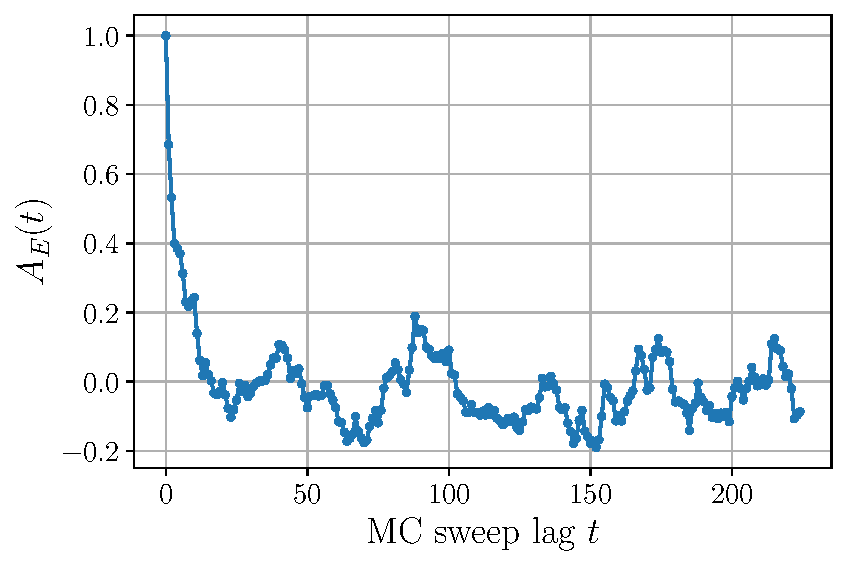
\includegraphics[width=\textwidth]{images/monte_carlo/autocorrfn.pdf}
    \end{subfigure}
    \caption{Exponential decay of energy density autocorrelation function.}
    \label{}
\end{figure}
%%% FIG %%%
\section{Expectation values and errors}
Once we have a set of uncorrelated Monte Carlo observable measurements, it is a simple task to calculate the mean and standard deviation of the uncorrelated observable measurement data $(|m|, e)$. However, for quantities that are not measured directly in the simulation but are computed as non-linear combinations of basic observables $(\chi, C_V, U_L)$, deriving a propagated error is a highly non-trivial task. Therefore, we utilize \textit{Jackknife analysis} to create large blocks/bins of the data and perform the required computations.

\subsection{Jackknife binning analysis}
We begin by binning the $N$ measurements of observable $\mathcal{O}$ into $N_B$ non-overlapping bins of length $k$ such that $N_B k = N$, and construct a shorter time series of bin averages. The bin average for the $j^\text{th}$ bin is defined as
\begin{equation}
    \mathcal{O}^{(B)}_j \equiv \frac{1}{k} \sum_{i = 0}^{k-1} \mathcal{O}_{jk+i} 
\end{equation}
Below is a visual representation of the binning process 
\begin{gather*}
    \{\underbrace{\{\mathcal{O}_0, \mathcal{O}_1 \ldots \mathcal{O}_{k-1}\}}_{\overline{\mathcal{O}}^{(B)}_0}, \underbrace{\{\mathcal{O}_{k}, \mathcal{O}_{k+1} \ldots \mathcal{O}_{2k-1}\}}_{\overline{\mathcal{O}}^{(B)}_1}, \ldots\ldots ,\underbrace{\{\mathcal{O}_{(N_B-1)k}, \mathcal{O}_{(N_B-1)k+1} \ldots \mathcal{O}_{N-1}\}}_{\overline{\mathcal{O}}^{(B)}_{N_B-1}}\} \\
    \Downarrow \\
    \{
        \overline{\mathcal{O}}^{(B)}_0, \overline{\mathcal{O}}^{(B)}_1, \overline{\mathcal{O}}^{(B)}_2 \ldots ,\overline{\mathcal{O}}^{(B)}_{N_B-1} 
    \}
\end{gather*}
Knowing the bin averages for the observables $\mathcal{O} \in \{\abs{m}, m^2, m^4, e, e^2 \}$, the bin estimates of the derived quantities are estimated as
\begin{equation}
    \chi^{(B)}_j = \beta \: L^2\:\qty(\overline{m^2}^{(B)}_j - \qty[\overline{|m|}^{(B)}_j]^2)
\end{equation}
\begin{equation}
    {C_V}^{(B)}_j = \beta ^2\: L^2 \:\qty(\overline{e^2}^{(B)}_{\:\:\:j} - \qty[\overline{e}^{(B)}_j]^2)
\end{equation}
\begin{equation}
    {U_L}^{(B)}_{\:\:\:j} = 1 - \frac{\overline{m^4}^{(B)}_j}{3\qty[\overline{m^2}^{(B)}_j]^2}
\end{equation}
% \begin{gather}
%     \chi^{(B)}_j = \beta \: L^2\:\qty(\overline{m^2}^{(B)}_j - \qty[\overline{|m|}^{(B)}_j]^2) \\[4pt] 
%     {C_V}^{(B)}_j = \beta ^2\: L^2 \:\qty(\overline{e^2}^{(B)}_{\:\:\:j} - \qty[\overline{e}^{(B)}_j]^2) \\
%     {U_L}^{(B)}_{\:\:\:j} = 1 - \frac{\overline{m^4}^{(B)}_j}{3\qty[\overline{m^2}^{(B)}_j]^2}
% \end{gather}
We denote these derived quantities by $\rho $ such that $\rho \in \{\chi , C_V, U_L\}$. The means over the bin averages (for $\mathcal{O}$) and bin estimates (for $\rho $) are also calculated
\begin{subequations}
    \begin{gather}
        \overline{\mathcal{O}} = \overline{\overline{\mathcal{O}}^{(B)}_j} = \frac{1}{N_B} \sum_{i=0}^{N_B-1} \overline{\mathcal{O}}^{(B)}_j \\
        \overline{\mathcal{\rho }} = \overline{{\rho }^{(B)}_j} = \frac{1}{N_B} \sum_{i=0}^{N_B-1} {\rho }^{(B)}_j
    \end{gather}       
    \label{binaverage} 
\end{subequations}
\!\!\!For the Jackknife error analysis, we begin by constructing the same number ($N_B$) of Jackknife bins containing all data but the $j^\text{th}$ bin of the previously mentioned binning method. The Jackknife averages for these new bins are defined as 
\begin{gather}
    \overline{\mathcal{O}}^{(J)}_j = \frac{N\overline{\mathcal{O}} - k \overline{\mathcal{O}}^{(B)}_j}{N - k} \\
    \overline{\rho }^{(J)}_j = \frac{N\overline{\rho } - k {\rho}^{(B)}_j}{N - k}
\end{gather}          
Since we are using the same data again and again while forming the Jackknife bins, these bins are trivially correlated, and as a result, the Jackknife bin variance is much smaller than is expected. This can be corrected by multiplying the sample variance by another factor of $(N_B-1)^2$ resulting in 
\begin{subequations}
    \begin{gather}
        \delta \overline{\mathcal{O}} = \sqrt{\frac{N_B-1}{N_B} \sum_{j=0}^{N_B-1}\qty(\overline{\mathcal{O}}^{(J)}_j - \overline{\mathcal{O}})^2} \\
        \delta \rho  = \sqrt{\frac{N_B-1}{N_B} \sum_{j=0}^{N_B-1}\qty(\overline{\rho }^{(J)}_j - \overline{\rho})^2}
    \end{gather}     
    \label{jackknifeerror}
\end{subequations}
\!\!\!Therefore, using the calculated values from Eq. \eqref{binaverage} and Eq. \eqref{jackknifeerror}, we get our mean and error estimates of the observable expectation values and the derived physical quantities
\[
    \text{Estimate of }\expval{\mathcal{O}} \rightarrow \overline{\mathcal{O}} \pm \delta \overline{\mathcal{O}}, \qquad\qquad \text{Estimate of }{\rho } \rightarrow \overline{\rho } \pm \delta {\rho } 
\]

\section{Critical slowing down}
Phase transitions, in general, are associated with a discontinuity in the first derivative (for first-order phase transitions) or a divergence in the second derivative (for second-order phase transitions). For example, the classical Ising model is characterized by a second-order phase transition at a critical temperature $T_c$. Above this temperature $(T>T_c)$, the spins are randomly aligned and correspond to the \textit{paramagnetic} phase. Below this temperature $(T<T_c)$, the spins majorly align in one of the directions to form the \textit{ferromagnetic} phase of the system.~\\~\\
%%% FIG %%%
\begin{figure}[!htb]
    \centering
    \begin{subfigure}[b]{0.4\textwidth}  %keep total sum <1 to show in same line
        \centering
        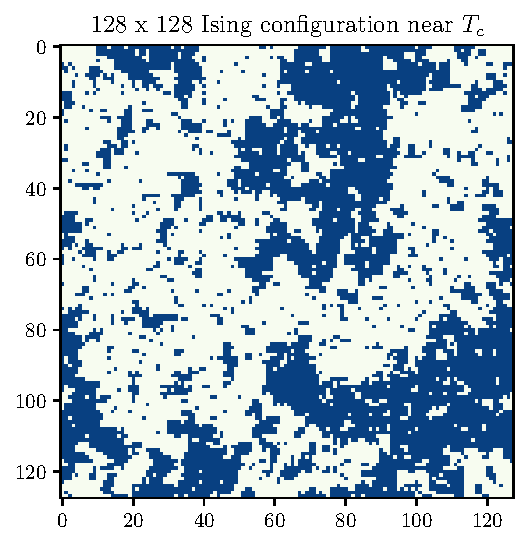
\includegraphics[width=\textwidth]{images/monte_carlo/ising_config_128.pdf}
        \caption{Domain formation near $T_c$ $(T=2.30)$.}
        \label{domain}
    \end{subfigure}
    \hspace{1em}  %\hfill
    \begin{subfigure}[b]{0.5\textwidth}
        \centering
        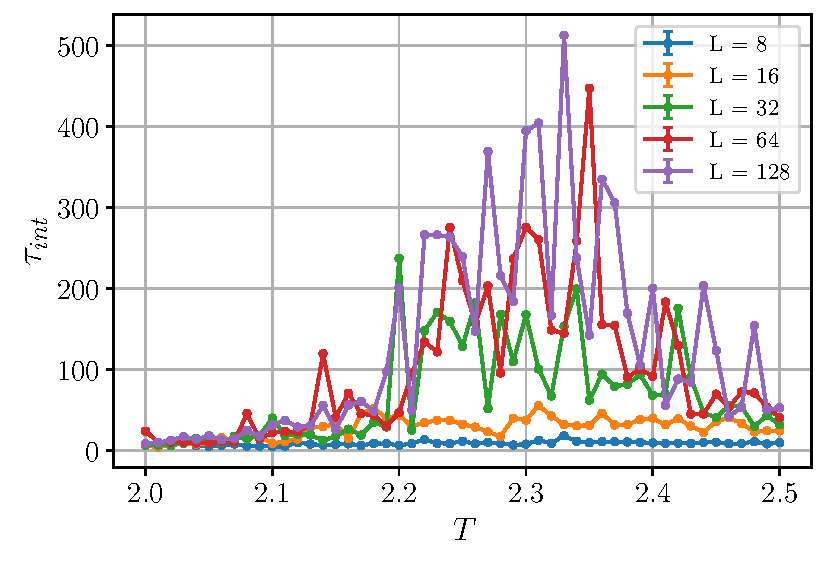
\includegraphics[width=\textwidth]{images/monte_carlo/metropolis_autocorr_time.pdf}
        \caption{High autocorrelation times near $T_c$ for Metropolis.}
        \label{autocorr_metropolis}
    \end{subfigure}
    \caption{Critical slowing down near the transition point in the Ising model.}
    \label{}
\end{figure}
%%% FIG %%%
% \FloatBarrier \!\!\!\!\!\!\!\!\!\!\!
\!\!\!In the paramagnetic phase, at high temperatures, the spin configuration is random and there are little to no spatial correlations. However, as the temperature decreases, we enter the paramagnetic phase and spins tend to align themselves with their neighbors. As a result, we form large \textit{domains} or \textit{clusters} of spins and we have a high degree of spatial correlation (Fig. \ref{domain}), often measured by the parameter $\xi$, known as the correlation length. As one approaches the critical temperature $T_c$ from the above, the onset of strong correlations results in \textit{domain flips} which cause high fluctuations in magnetization and energy. Since the Metropolis algorithm performs local updates and the spins have a strong spatial correlation, we need to wait for a long autocorrelation time to get independent subsequent measurements (Fig. \ref{autocorr_metropolis}). This is known in literature as \textit{critical slowing down}.~\\~\\
The phenomena of critical slowing down is primarily dependent on the algorithm used. Since local update (such as Metropolis) take a long time to flip the domains and generate statistically independent configurations, they have a significantly higher computational cost as a tradeoff to their conceptual simplicity.~\\~\\
Therefore, it should be intuitively clear that some sort of non-local updates should be able to alleviate this problem by flipping entire clusters of spins. This class of algorithms is generally known as \textit{Cluster-update algorithms}. Although the critical slowing down can be significantly reduced with cluster algorithms, they are still far less general applicable than local update algorithms.

\section{Wolff Cluster algorithm}
The acceptance probability of local update algorithms is very low around the critical regions making it an inefficient way to probe the critical properties of the system. In this section, we will discuss the \textit{Wolff cluster algorithm}, which is a generalization of the Swendsen-Wang clyster dynamics and is even more efficient. The Wolff cluster algorithm works by identifying domains of identically oriented spins and performing a flip operation on the entire cluster [Krauth].
\subsection{Deriving the probabilities}
We will start by considering the example of two states $a$ and $b$ which differ by flipping of a cluster of identically oriented spins.~\\~\\
This can be done by starting the construction of a cluster which starts by seeding a random spin and iteratively adding neighboring sites of the same spin with a probability $p$. This means if a spin $i$ is in the cluster, and a neighboring site $j$ is not (and if $\sigma_i = \sigma_j$), then the link $\expval{i,j}$ should be added into the cluster with a probability $p$. Once the construction has stopped, we will still have $n_\text{same}$ identical spin links just outside the cluster boundary which were not added into the cluster. Similarly, we say the number of opposite spin links which have a spin opposite to that of the cluster is $n_\text{opp}$. Also, $n_\text{same} + n_\text{opp} = N$ where $N$ is the total number of links the cluster makes with outside spins.~\\~\\  
Since the probability of a site not being accepted into the cluster is $(1-p)$, the ``a-priori'' probability of proposing a cluster flip from $a \to b$ is 
\begin{equation}
    \mathcal{A}(a \to b) = \mathcal{A}_\text{interior} \cdot (1-p)^{n_\text{same}},
\end{equation}
where $\mathcal{A}_\text{interior}$ is just a product of probabilities for links that were accepted into the cluster. In the reverse direction, if we would have started with the state $b$ and tried constructing a cluster and flipping it to go to state $a$, the ``a-priori'' probability to propose a cluster flip from $b \to a$ is 
\begin{equation}
    \mathcal{A}(b \to a) = \mathcal{A}_\text{interior} \cdot (1-p)^{n_\text{opp}}
\end{equation}
because in state $b$, the unaccepted but identical spins were exactly those which had the opposite spin in state $a$. Therefore, if we invoke the detailed balance condition Eq. \eqref{detailedbalance} for the cluster flips to get
\begin{equation}
    \frac{\mathcal{A}(a \to b) \cdot P_\text{accept}(a \to b)}{\mathcal{A}(b \to a) \cdot P_\text{accept}(b \to a)} = e^{-\beta(E_b - E_a)}
\end{equation}
Now the energies of states $a$ and $b$ can be computed as nearest neighbor interaction \textit{inside the cluster} and the interaction \textit{outside the cluster}. Since $a$ and $b$ only differ by a cluster flip, the only difference appears in the interaction at the cluster boundary
\begin{subequations}
    \begin{gather}
        E_a = E_\text{interior} + E_\text{exterior} - n_\text{same}J + n_\text{opp} J, \\
        E_b = E_\text{interior} + E_\text{exterior} - n_\text{opp}J + n_\text{same} J \\ 
        \implies E_b - E_a = 2J(n_\text{same} - n_\text{opp})
    \end{gather}
\end{subequations}
Therefore, putting in the expressions into the detailed balance condition, we get
\begin{subequations}
    \begin{gather}
        \frac{P_\text{accept}(b \to a)}{P_\text{accept}(a \to b)} = e^{-2\beta J(n_\text{same} - n_\text{opp})} (1-p)^{n_\text{opp} - n_\text{same}} \\
        \implies \frac{P_\text{accept}(b \to a)}{P_\text{accept}(a \to b)} = \qty(\frac{e^{-2\beta J}}{1-p})^{n_\text{same} - n_\text{opp}}
    \end{gather}
\end{subequations}
Thus, given a value of $p$ (which can be a function of $\beta$ and $J$), we can get the corresponding acceptance probability for the cluster algorithm. An interesting coincidence occurs when 
\begin{equation}
    p = 1 - \exp(-2\beta J).
\end{equation}
This special choice of probability function yields a \textit{rejection-free} algorithm whose acceptance probability is always 1. 
\begin{equation}
    \eval{\frac{P_\text{accept}(b \to a)}{P_\text{accept}(a \to b)}}_{p = 1 - \exp(-2\beta J)} = \qty(\frac{e^{-2\beta J}}{e^{-2\beta J}})^{n_\text{same} - n_\text{opp}} = 1
\end{equation}
Thus, any proposed cluster construction and flipping is an always accepted move in the cluster algorithm. The cluster algorithm with the particular choice of $p = 1 - e^{-2\beta J}$ is known as the Wolff cluster algorithm. 

\subsection{Implementation}
In this subsection, we will try to discuss an algorithmic implementation of Wolff clusters so that it can be easily coded into a Monte Carlo program.~\\~\\
Before starting, we will assume we are working with a 2-dimensional spin configuration and we aim to generate configurations distributed according to the Boltzmann distribution using Monte Carlo evolution with transition probabilities given by the Wolff scheme, which is the fastest currently known simulation method for the Ising model. One Wolff algorithm step is then defined in the following step-by-step procedure,
\begin{enumerate}
    \setlength\itemsep{0.3em}
    \item Randomly choose a site $i$ on the lattice with the spin $\sigma_i$.
    \item Label the neighbors of $i$ as $j$. Add them to a temporary set. Call this set $N_\text{temp}$. 
    \item If $\sigma_i = \sigma_j$, add the neighbor $j$ from set $N_\text{temp}$ to the cluster $\mathcal{C}$  with a probability of $p = 1 - e^{-2\beta J}$.
    \item Repeat step 2 for all the neighbors in set $N_\text{temp}$.
    \item For sites that are \textit{newly added} to the cluster, check for neighboring identical spins and add them to the cluster $\mathcal{C}$ by repeating steps 2 to 4.
    \item Keep repeating till no more spins are added to the cluster $\mathcal{C}$.
    \item Once the cluster is constructed, flip all the spins, i.e., $\forall \:j \: \in \mathcal{C} \: | \: \sigma_j \to - \sigma_j$.
\end{enumerate}
More concisely, a single sweep of the Monte Carlo Wolff algorithm in \texttt{psuedocode language} is given below from [Krauth]. The sets $\mathcal{F}_\text{old}$ and $\mathcal{F}_\text{new}$ denote the frontier of the cluster at $(n-1)^\text{th}$ and $n^\text{th}$ steps, respectively. The set $\mathcal{C}$ contains the sites belonging to the cluster.~\\~\\
\begin{algorithm}{wolff-cluster}
    \> $i:=\text{random site}$; \\
    \> $\mathcal{C}:=\{ i \}$; \\
    \> $\mathcal{F}_{\text{old}}:=\{i \};$\\
    \>{\bf while} $\mathcal{F}_{\text{old}} \neq \{ \}$ {\bf do}\\
    \>{\bf begin}\\
    \>\> $\mathcal{F}_{\text{new}}:=\{ \};$\\
    \>\>{\bf for} $\forall\ i\ \in\ \mathcal{F}_{\text{old}}$ {\bf do}\\
    \>\>{\bf begin}\\
    \>\>\>{\bf for} $\forall\ j\ \text{neighbor of $i$ with $\sigma_i=\sigma_j$},\ j
     \not \in \mathcal{C} $ {\bf do}\\
    \>\>\>{\bf begin}\\
    \>\>\>\>{\bf if} $\text{ran}[0,1] < p$ {\bf then}\\
    \>\>\>\>{\bf begin}\\
    \>\>\>\>\>$\mathcal{F}_{\text{new}}:= \mathcal{F}_{\text{new}}\cup \{j\};$\\
    \>\>\>\>\>$\mathcal{C}:= \mathcal{C} \cup \{j\};$\\
    \>\>\>\>{\bf end}\\
    \>\>\>{\bf end}\\
    \>\>{\bf end}\\
    \>\>$\mathcal{F}_{\text{old}}:= \mathcal{F}_{\text{new}};$\\
    \>{\bf end}\\
    \>{\bf for} $\forall\ i\ \in\ \mathcal{C}$ {\bf do}\\
    \>$\sigma_i:= -\sigma_i;$\\
\end{algorithm}
The resulting dynamics is ergodic and obeys detailed balance.
\section{Results}
We have now setup our complete machinery for calculating physical observable expectation values (and errors) using Monte Carlo Wolff algorithm simulations. The workflow of the Monte Carlo code is summarized in the following section.

\subsection{Structure of the code}
The \texttt{ising} executable program calculates the expectation values of various observables and physical quantities derived from them, along with error bars. Each iteration of the program runs for a single $(L, T)$ pair. The program is structured into four parts
\begin{itemize}[label={}]
    \item \textbf{Part 1} \:\:\: A preliminary Monte Carlo run to collect autocorrelated observable measurements after the system equilibrates.
    \item \textbf{Part 2} \:\:\: Calculation of the integrated autocorrelation time $\tau_\text{int}$ using the autocorrelated measurements. 
    \item \textbf{Part 3} \:\:\: The main Monte Carlo run with observable measurements being taken after every $2\tau_\text{int}$ MC sweeps to ensure collection of uncorrelated measurements.
    \item \textbf{Part 4} \:\:\: Calculating observable expectation values and derived physical quantities with error bars using jackknife binning method.  
\end{itemize} 
After obtaining the results of expectation values and derived physical quantities (with error bars) for a range of temperatures, we perform finite-size scaling analysis on the data to extract the critical exponents of the 2D Ising Model. The \texttt{ising-2d} source code is written in \texttt{C++} and the files can be accessed on the following link - \href{https://github.com/kunal1729verma/ising-2d}{\texttt{ising-2d} on GitHub}.

\subsection{Simulation results}
The following parameters were used in the 2D Ising model simulations for lattice sizes of $L = 8, 16, 32, 64, 128$. Here, we have used the Wolff scheme to simulate the Markov chain Monte Carlo procedure instead of the Metropolis algorithm for reasons discussed in earlier sections. As a short remark on units, we are using the natural units where $k_B = 1$, so our units of temperature and energy are identical. We have also set the coupling paramater as unity \texttt{J = 1.0}.
\begin{itemize}[label={}]    
    \setlength{\itemsep}{0.1em}
    \item \textbf{For preliminary Monte Carlo (Part 1)}
    \begin{itemize}[label={}] 
        \setlength{\itemsep}{0.1em}   
        \item \texttt{no of equilibration sweeps = 1.0e3}
        \item \texttt{no of sampling sweeps = 1.0e4}
        \item \texttt{sampling step size = 1.0e0}
    \end{itemize} 
    \item \textbf{For the main Monte Carlo run (Part 3)}
    \begin{itemize}[label={}]    
        \setlength{\itemsep}{0.1em}
        \item \texttt{no of equilibration sweeps = 1.0e3}
        \item \texttt{no of sampling sweeps = 2$\tau \: \cdot$ 2.0e4}
        \item \texttt{sampling step size = 2$\tau $ }
    \end{itemize} 
\end{itemize}
%%% FIG %%%
\begin{figure}[!htb]
    \centering
    \begin{subfigure}[b]{0.49\textwidth}  %keep total sum <1 to show in same line
        \centering
        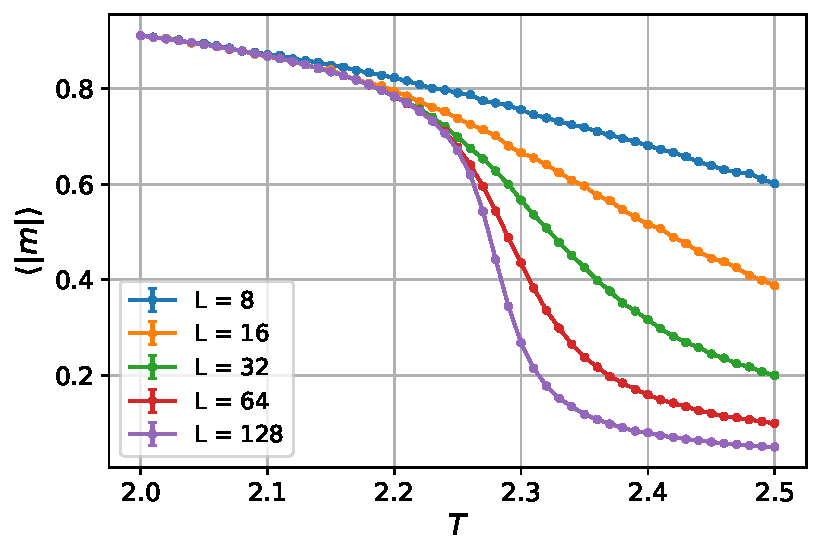
\includegraphics[width=\textwidth]{images/monte_carlo/wolff_cluster/abs(mag).pdf}
        \caption{$\expval{\abs{m}} \text{ vs } T$}
        \label{magnetization}
    \end{subfigure}
    % \hspace{1em}  %\hfill
    % \vspace{1em}
    \begin{subfigure}[b]{0.49\textwidth}
        \centering
        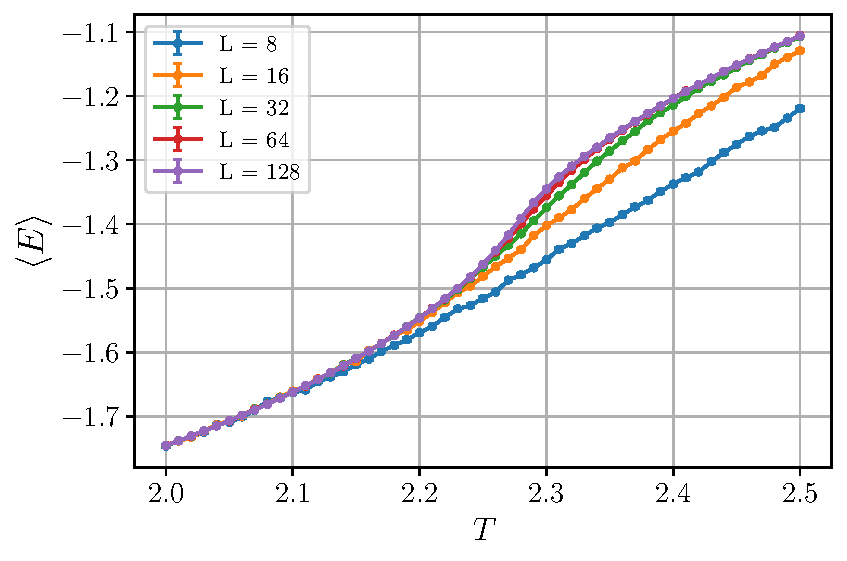
\includegraphics[width=\textwidth]{images/monte_carlo/wolff_cluster/edens.pdf}
        \caption{$\expval{e} \text{ vs } T$}
    \end{subfigure}
\end{figure}
%%% FIG %%%
%%% FIG %%%
\begin{figure}[!htb]\ContinuedFloat
    \centering
    \begin{subfigure}[b]{0.49\textwidth}
        \centering
        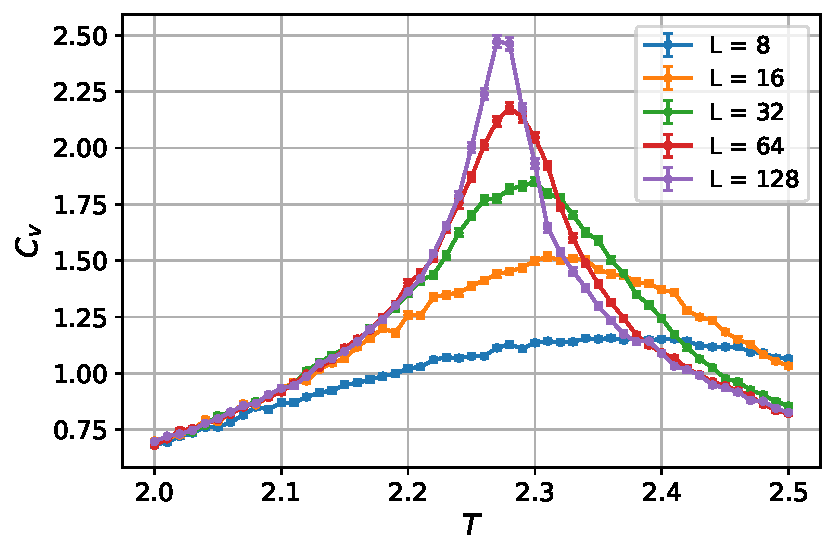
\includegraphics[width=\textwidth]{images/monte_carlo/wolff_cluster/C_v.pdf}
        \caption{$C_V \text{ vs } T$}
        \label{specificheat}
    \end{subfigure}
    % \hspace{1em}  %\hfill
    \begin{subfigure}[b]{0.49\textwidth}
        \centering
        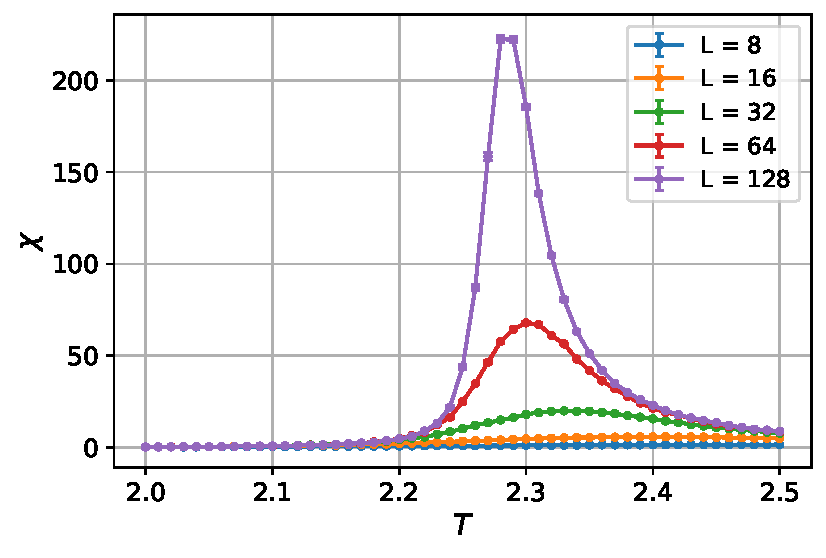
\includegraphics[width=\textwidth]{images/monte_carlo/wolff_cluster/chi.pdf}
        \caption{$\chi \text{ vs } T$}
        \label{susceptibility}
    \end{subfigure}
\end{figure}
%%% FIG %%%
%%% FIG %%%
\begin{figure}[!htb]\ContinuedFloat
    \centering
    \begin{subfigure}[b]{0.49\textwidth}
        \centering
        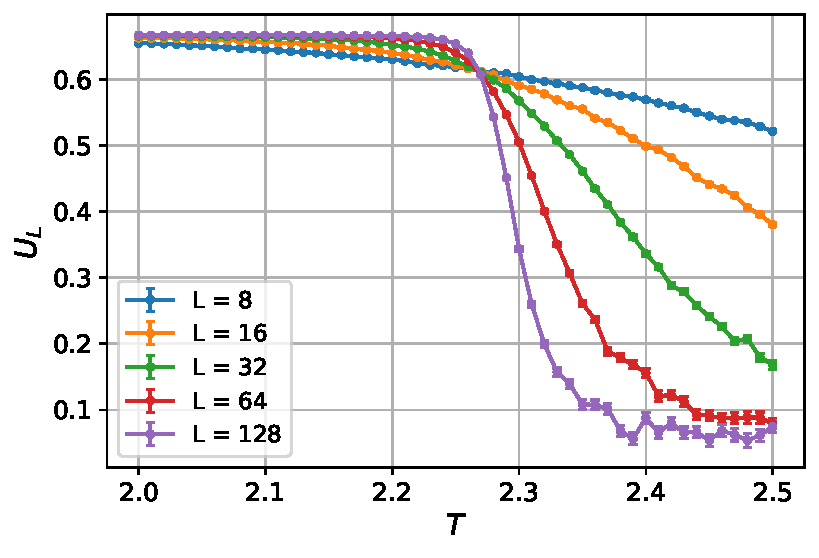
\includegraphics[width=\textwidth]{images/monte_carlo/wolff_cluster/U_L.pdf}
        \caption{$U_L \text{ vs } T$}
        \label{bindercumulant}
    \end{subfigure}
    % \hspace{1em}  %\hfill
    \begin{subfigure}[b]{0.49\textwidth}
        \centering
        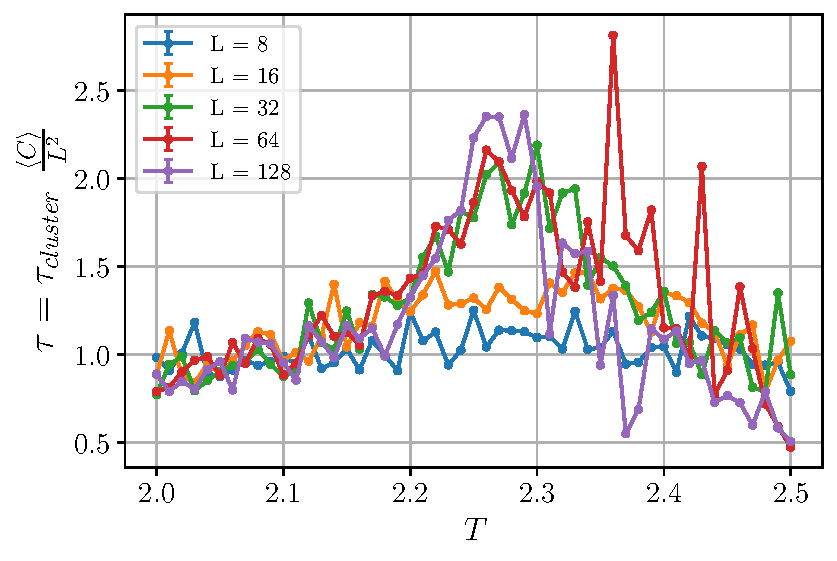
\includegraphics[width=\textwidth]{images/monte_carlo/wolff_cluster/autocorr times.pdf}
        \caption{$\tau_\text{int} \text{ vs } T$}
        \label{autocorrelationtime}
    \end{subfigure}
    \caption{Variation of physical quantities with $T$ for different lattice sizes $L$.}
    \label{expvalvsT}
\end{figure}
%%% FIG %%%
\FloatBarrier \!\!\!\!\!\!\!\!\!\!\!\!
The Figure \ref{expvalvsT} above shows plots of expectation values of relevant observables, derived physical quantities and the autocorrelation times (scaled by $\expval{C}/L^2$) as they vary with $T$ for different lattice sizes $L$. These plots summarize the entire critical structure of Ising model tansition.~\\~\\
The average (absolute) magnetization curve as a function of temperature (Fig. \ref{magnetization}) is one of the most interesting results of the Ising model. The average (absolute) magnetization is the order parameter for the Ising model which distinguishes the paramagnetic and ferromagnetic phases of the model. As we go to higher and higher lattice sizes, the transition points becomes progressively sharper and shows a clear transition from ferromagnetism $(\expval{|m|} \approx 1)$ to paramagnetism $(\expval{|m|} \approx 0)$ after a certain transition temperature $T_c$ at $L = 128$.~\\~\\
Another interesting feature of the Ising phase transitions are the specific heat $C_V$ (Fig. \ref{specificheat}) and magnetic susceptibility $\chi$ (Fig. \ref{susceptibility}) curves. They show an approximate divergence at the critical temperature $T_c$, which becomes exact in the thermodynamic limit $L \to \infty$. Hence, our numerical studies confirm that the Ising phase transition is second-order in nature.~\\~\\
The way to numerically estimate the critical temperature $T_c$ of the phase transition was given by Binder [Binder 1981]. According to Binder, the transition temperature $T_c$ is the temperature at which different $U_L$ curves (corresponding to different lattice sizes $L$) cross in the thermodynamic limit (Fig. \ref{bindercumulant}). In our studies, we estimated the critical temperature $T_c \approx 2.269$, which is very close to the exact value of $2/\ln\qty(1+\sqrt{2}) \approx 2.26918$.~\\~\\
Finally, a short note on autocorrelation times. As one can see in Fig. \ref{autocorrelationtime}, we have scaled the $\tau_\text{cluster}$ by $\expval{C}/L^2$, where $\expval{C}$ is the average cluster size. We claim that this is the correct autocorrelation time to compare with the Metropolis autocorrelation times [Tamayo et al]. This is because $N$ Metropolis sweeps are fundamentally different than $N$ Wolff sweeps. If we go through $N$ sweeps, 
\begin{gather*}
    \text{For Metropolis } \longrightarrow N \cdot L^2 \text{ spin flips} \\
    \text{For Wolff cluster } \longrightarrow N \cdot \expval{C} \text{ spin flips}
\end{gather*}
So if we were to define an equivalent unit of time as $(\text{\# of spin flips})/L^2$, then for $N$ sweeps
\begin{gather*}
    T_\text{Metro} = \frac{N \cdot L^2}{L^2} = N \\
    T_\text{Wolff} = N \frac{\expval{C}}{L^2}
\end{gather*}     
Hence, we also scale our Wolff autocorrelation time $\tau_\text{cluster}$ by a factor of $\expval{C}/L^2$, and we can see in Fig. \ref{autocorrelationtime} that it's much more efficient compared to the Metropolis algorithm (Fig. \ref{autocorr_metropolis}). Further, the autocorrelation times are observed to scale with system size as a power law 
\[
    \tau_\text{int} \sim L^z
\]
where $z$ is the dynamical critical exponent, and can be used to quantify the efficiency of the algorithm. We will, however, not go in that direction and instead focus on the remaining critical exponents which characterize the Ising phase transition. 

\section{Critical phenomena and Finite-size scaling}
We will now give a brief review of critical phenomena and the finite-size scaling properties that can be quantitatively used to study critical properties of the problem using Monte Carlo simulations. In general, phase transitions only happen in the thermodynamic limit $(L  \infty)$. However, since we only possess finite computational memory and processing time, it is not possible to numerically simulate arbitrarily large system sizes to study the critical properties of a system. Therefore, we use the theory of \textit{finite-size scaling analysis} which uses the results for finite system sizes to deduce conclusions for the thermodynamic limit. 
\subsection{Critical Exponents}
The critical phenomena are generally scaling forms that occur near the critical point. For the classical Ising model, we obtain scaling relations for observable expectations near the classical critical point, i.e., the critical temperature $T_c$. As mentioned earlier, we can use the data from finite-size studies to estimate the critical exponents using the \textit{data-collapse method}. However, this analysis is only possible for second-order phase transitions and it fails for first-order transitions. ~\\~\\
The most fundamental concept underlying the theory of critical phenomena is that of a \textit{correlation length}, denoted by $\xi$. It roughly denotes the typical size of ordered domains in the lattice. Close to the critical point $T_c$, the correlation length diverges according to a power law
\begin{equation}
    \xi \sim t^{-\nu},
\end{equation}
where $t$ is defined as the reduced temperature 
\begin{equation}
    t \equiv \frac{|T-T_c|}{T_c},
\end{equation}
and $\nu$ is one of the critical exponents, and is the same whether we approach $T_c$ from above or below. Similarly, the critical exponent corresponding to the onset of magnetic order is given by $\beta$. The order parameter $\expval{|m|}$ is zero above $T_c$, and below $T_c$ it scales as
\begin{equation}
    \expval{|m|} \sim t^\beta \quad (\sim \xi^{-\beta/\nu})
\end{equation}
The susceptibility, as noted previously, diverges at $T_c$ in the thermodynamic limit and scales as 
\begin{equation}
    \chi \sim t^{-\gamma} \quad (\sim \xi^{\gamma/\nu})
\end{equation} 
The specific heat is also diverges from both above and below as it approaches $T_c$ 
\begin{equation}
    C_V \sim t^{-\alpha} \quad (\sim \xi^{\alpha/\nu})
\end{equation}
It is, however, to be noted that the above scaling relations near the critical point hold true in the infinite size limit $(L \to \infty)$. Systems belonging to the same \textit{universality class} have the same set of critical exponents $\{ \nu, \beta, \gamma, \delta, \alpha \}$. The universality class does not depend on the microscopic details but instead on the behavior of the system near the critical point.

\subsection{Finite-size scaling hypothesis}
How would the scaling relations modify if the lattice sizes $L$ are finite? The order parameter $\expval{|m|}$ does not exactly vanish for $T \geq T_c$, and the divergent quantities (like $\chi$ and $C_V$) saturate to a finite value.~\\~\\
One possible way is to perform finite-size simulations for higher and higher $L$ until the results converge, and extract the critical exponents by estimating the exponent in the power law. However, a much more systematic way is to perform a \textit{finite-size scaling} (FSS) study which uses the regularity in the deviations to extract the critical exponents.~\\~\\
Consider the susceptibility in an infinite size limit which scales as 
\[
   \chi \sim \xi^{\gamma/\nu}
\]
Then the \textit{finite-size scaling hypothesis} (which can be proven via renormalization group theory) states that observables close to $T_c$ scale with an additional non-divergent function of $\xi/L$ to account for the deviations in critical behavior at finite sizes
\begin{equation}
    \chi(\xi, L) = \xi^{\gamma/\nu} \: f(\xi/L)
\end{equation}
where $f(x) \to $ const. as $x \to 0$ ($L \to \infty$). Since the deviations from the $L \to \infty$ critical behavior occurs when the correlation length $\xi$ is comparable to the system size $L$, and the fact that $\xi \sim t^{-\nu}$, we obtain the much more familiar expression of the FSS hypothesis 
\begin{equation}
    \chi(t, L) = L^{\gamma/\nu} \: g(t L^{1/\nu})
\end{equation}
where $g$ is another scaling function. More generally, for any observable (or derived quantity) $Q$, the quantity scales as
\begin{equation}
    Q(t, L) = L^{\zeta/\nu} \: g_Q(t L^{1/\nu})
\end{equation}
where $\zeta$ is the critical exponent corresponding to the scaling of the quantity $Q$.  
\begin{gather}
    \text{\textbf{Finite-size scaling relations for 2D Ising model} } \\
    U_L =\:\:\: \: g_U(t L^{1/\nu}) \nonumber \\ 
    |m| = L^{-\beta/\nu} \: g_{m}(t L^{1/\nu}) \nonumber \\
    \chi = L^{\gamma/\nu} \: g_\chi(t L^{1/\nu}) \nonumber \\
    C_V = \ln(L) \: g_C(t L^{1/\nu}) \nonumber
\end{gather}
In the case of the 2D Ising model, $\alpha = 0$, and hence the power law scaling doesn't hold. Instead, we have a logarithmic scaling as indicated in the scaling of $C_V$ as shown above.

\subsection{Data collapse method}
Since the master curve $g_Q(x)$ for a quantity $Q$ is an unknown function, one can plot $Q(t, L) \:L^{-\zeta/\nu}$ versus $x = tL^{1/\nu}$ for different sizes to extract the master curve. If the finite-size scaling hypothesis is correct, data for all the different lattice sizes should \textit{collapse} onto each other. However, this would require inputting the correct value of the critical exponents $\zeta$ and $\nu$.~\\~\\
Therefore, the problem of \textit{estimating the critical exponents} can be rephrased as a data collapse problem of the observable data ($Q(t, L) \:L^{-\zeta/\nu}$ versus $x = tL^{1/\nu}$) by fine-tuning the exponents $\zeta$ and $\nu$. We use the following cost function $P_b$ to as a measure of the collapse, which is essentially a normalized sum of residues, which we get by slightly modifying the cost function given in \cite{Bhattacharjee_2001}.
\begin{equation}
    P_b = \frac{1}{N_\text{over}} \sum_p \sum_{j \neq p} \sum_i \frac{\qty|L_j^{-\zeta/\nu}Q_{ij} - \varepsilon_p\qty(L_j^{1/\nu} t_{ij})|}{L_j^{-\zeta/\nu}Q_{ij} + \varepsilon_p\qty(L_j^{1/\nu} t_{ij})}
\end{equation}    
\begin{itemize}[label={\textbf{--}}]
    \setlength{\itemsep}{0.1em}
    \item $p$ indexes the data-set associated to length $L_p$. 
    \item $j$ also indexes the data-set associated to length $L_j$, but doesn't include the set $p$.      
    \item $i$ indexes the data-points inside the set associated to $L_j$.
    \item $N_\text{over}$ is the number of terms we sum over. 
    \item $\varepsilon_p$ is the interpolating function based on the values of set $p$ bracketing the argument in question. 
\end{itemize} 
The critical exponents are obtained by minimizing the cost funtion $P_b$ with respect to $\beta, \gamma, \nu$
\begin{itemize}[label={\textbf{--}}]
    \setlength{\itemsep}{0.1em}
    \item $Q = U_L$, minimize $P_b(0, \nu)$ with respect to $\nu$. $\:\:\quad\quad\quad\longrightarrow \nu_0$
    \item $Q = \expval{|m|}$, minimize $P_b(-\beta, \nu_0)$ with respect to $\beta$. $\quad\longrightarrow \beta_0$
    \item $Q = \chi$, minimize $P_b(\gamma, \nu_0)$ with respect to $\gamma$. $\:\:\quad\quad\quad\longrightarrow \gamma_0$   
\end{itemize}
The data collapse of the quantities obtained from the Monte Carlo studies is shown in Fig. \ref{datacollapse}. The appropriate fine-tuning of the critical exponents results in an almost perfect collapse of the data near the critical point $t = 0$.
%%% FIG %%%
\begin{figure}[!htb]
    \centering
    \begin{subfigure}[b]{0.49\textwidth}  %keep total sum <1 to show in same line
        \centering
        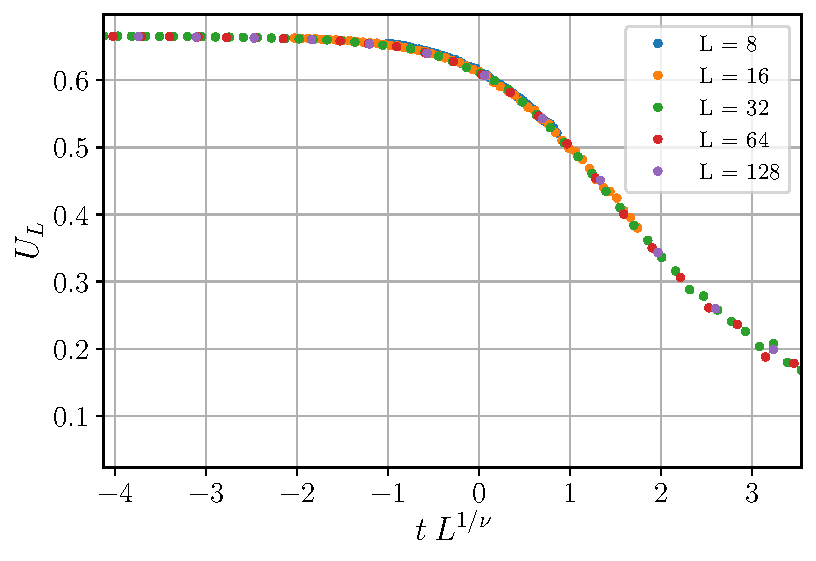
\includegraphics[width=\textwidth]{images/data collapse/U_L data collapse.pdf}
        \caption{Data collapse for $U_L$.}
        \label{U_L collapse}
    \end{subfigure}
    % \hspace{1em}  %\hfill
    % \vspace{1em}
    \begin{subfigure}[b]{0.49\textwidth}
        \centering
        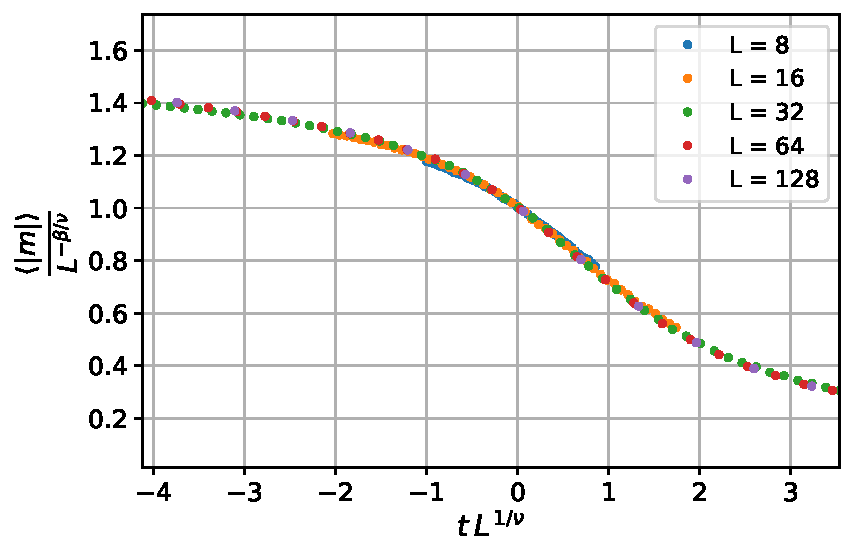
\includegraphics[width=\textwidth]{images/data collapse/abs(mag) data collapse.pdf}
        \caption{Data collapse for $\expval{\abs{m}.}$}
    \end{subfigure}
\end{figure}
%%% FIG %%%
%%% FIG %%%
\begin{figure}[!htb]\ContinuedFloat
    \centering
    \begin{subfigure}[b]{0.49\textwidth}
        \centering
        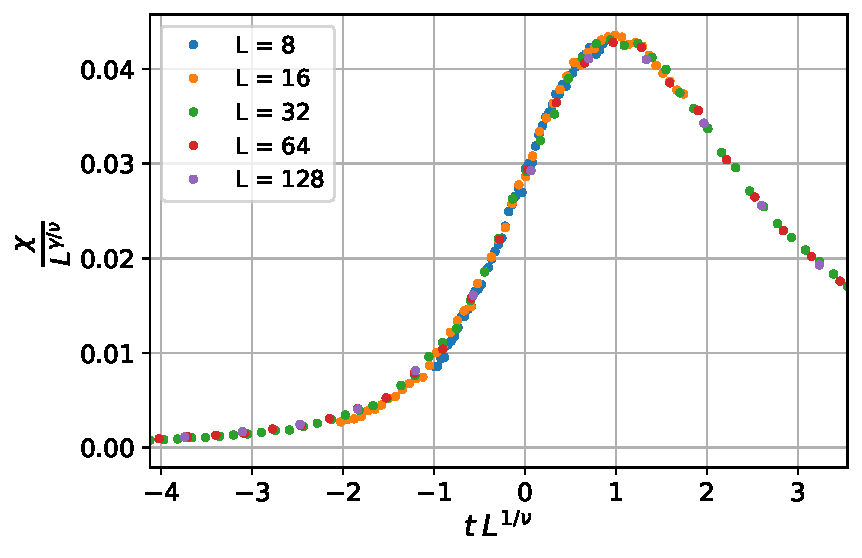
\includegraphics[width=\textwidth]{images/data collapse/chi data collapse.pdf}
        \caption{Data collapse for $\chi$.}
        \label{chi collapse}
    \end{subfigure}
    % \hspace{1em}  %\hfill
    \begin{subfigure}[b]{0.49\textwidth}
        \centering
        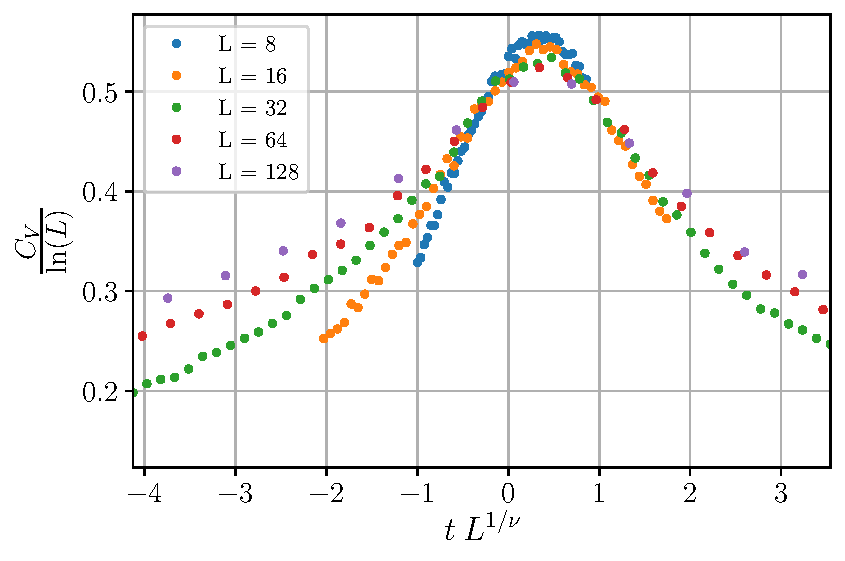
\includegraphics[width=\textwidth]{images/data collapse/C_v data collapse.pdf}
        \caption{Data collapse for $C_V$.}
        \label{C_V collapse}
    \end{subfigure}
    \caption{Data-collapse to extract the critical exponents.}
    \label{datacollapse}
\end{figure}
%%% FIG %%%
\FloatBarrier \!\!\!\!\!\!\!\!\!\!\!
The following table (Table \ref{critical}) summarizes the results of the critical exponents computed from a finite-size scaling study of the data obtained from Monte Carlo simulations compared to the exact values.
%%% TABLE %%%
\begin{table}[h!]
    \begin{center}
    \begin{tabular}{||c c c c||}
    \hline
    Physical Quantity & Exponent & FSS estimate  & Exact Value \\ \hline\hline
    Specific Heat ($C_V$) & $\alpha$ & \textbf{--} & 0 \\ \hline
    Order Parameter ($\expval{|m|}$) & $\beta$ & 0.1204 & 1/8 \\ \hline
    Magnetic Susceptibility ($\chi$) & $\gamma$ & 1.7301 & 7/4 \\ \hline
    Correlation Length ($\xi$) & $\nu$ & 0.9765 & 1 \\ \hline
    Critical Temperature & $T_c$ & 2.269  & $2/\ln(1+\sqrt{2})$ \\
    \hline
    \end{tabular}
    \caption{Summary of critical exponents for the 2D Ising model.}
    \label{critical}
    \end{center}   
\end{table}
%%% TABLE %%%
\section{What now?}
In this chapter, we provided a comprehensive introduction for implementing Monte Carlo simulations to classical spin system models. We explicitly discussed the example of the 2D Ising model, constructed both local and cluster update algorithm to compute expectation values of the observables, and described the framework of extracting the critical exponents via finite-size scaling analysis. This methodology can further be extended to other spin models for computing the critical properties near second-order phase transitions. Moreover, in the upcoming chapters, we'll discuss a scheme to generalize this approach to quantum spin models and use \textit{Quantum Monte Carlo} methods to explore the critical properties of the quantum phase transition. 
\end{document}